\section{Current-Starved Delay Stage Details}
\label{app:cs_delay_details}

Figure~\ref{fig:current_starved_delay_stage} shows the chain of six inverters used in the original clock deskew delay path. Four programmable stages combine a digitally controlled tri-state inverter with a current-starved inverter. The pull-up and pull-down branches are independently biased, enabling duty-cycle correction.

The bias voltages are generated by diode-based \gls{dac}s. Each \gls{dac} resembles an inverter with an enable signal controlling an NMOS and PMOS pair; series-connected diodes set the effective strength of each branch. Multiple \gls{dac} cells share an output node whose voltage adjusts the current limits of the current-starved inverters, thereby tuning the delay.

\begin{figure}[htbp]
  \centering
  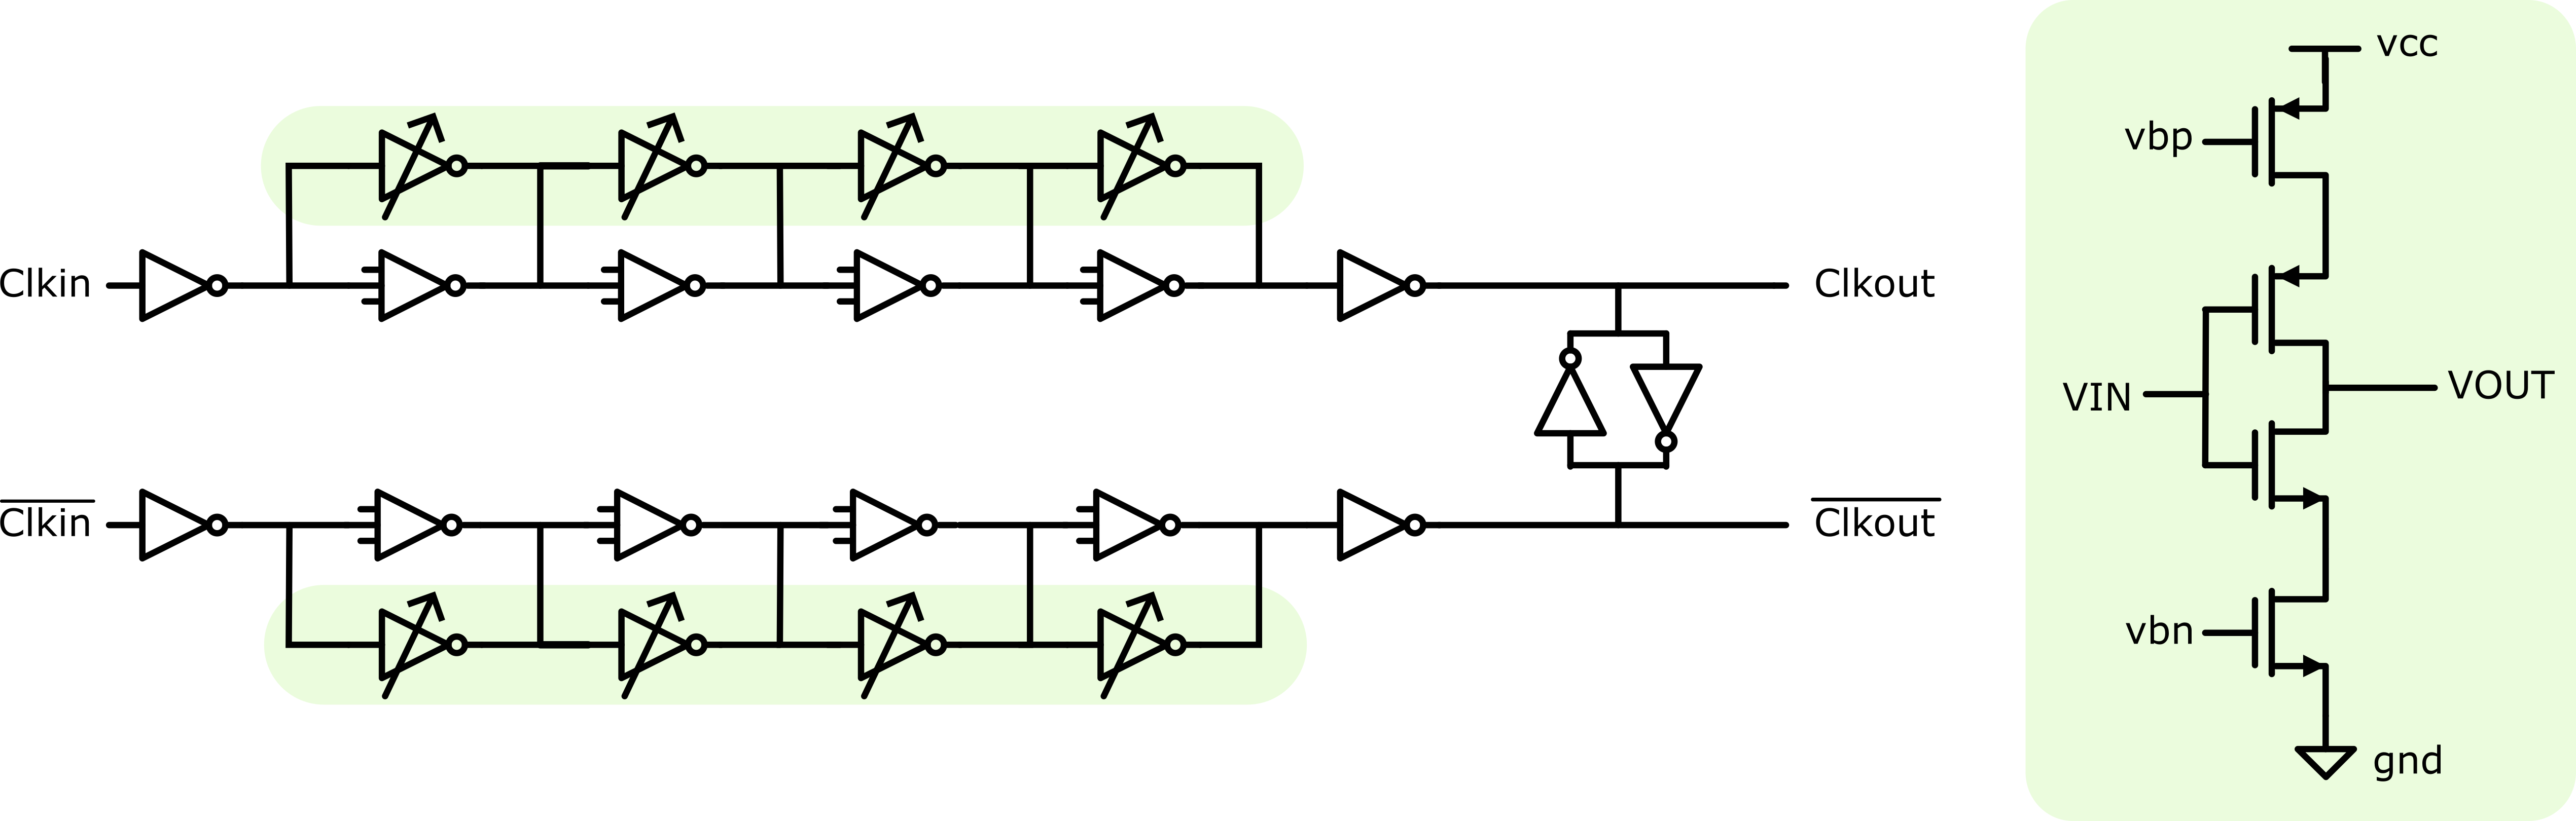
\includegraphics[width=0.8\linewidth]{figures/Schematics/old_chain.png}
  \caption{Current-starved delay stage with programmable inverters.}
  \label{fig:current_starved_delay_stage}
\end{figure}

\begin{figure}[htbp]
  \centering
  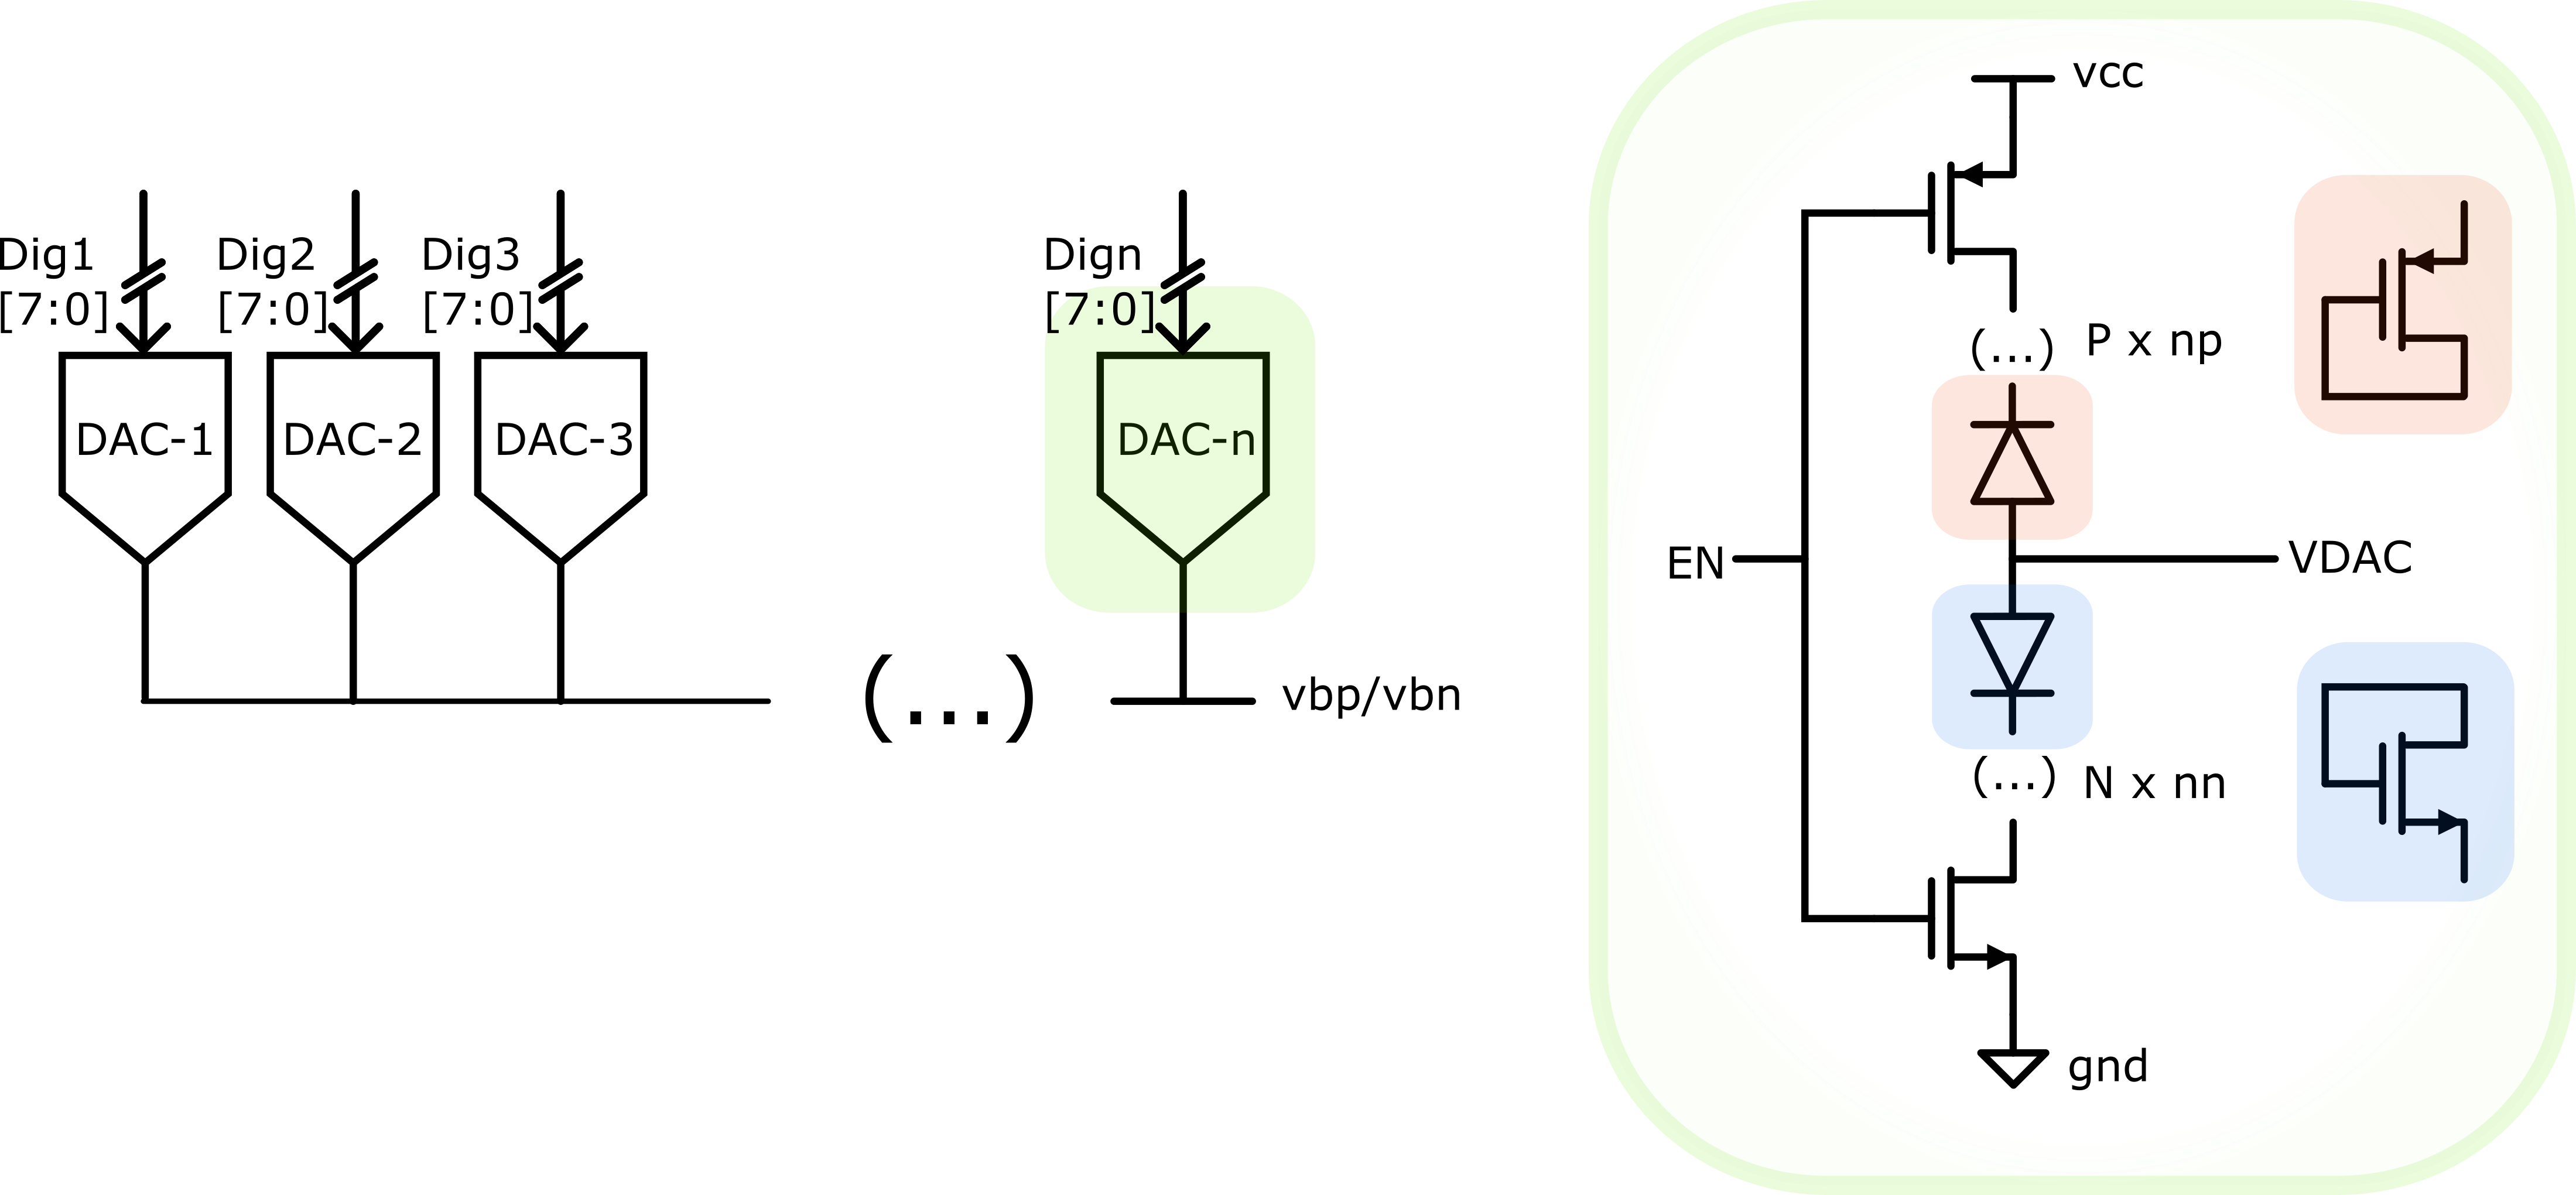
\includegraphics[width=0.8\linewidth]{figures/Schematics/old_DAC.png}
  \caption{Current-starved DAC used for biasing the current-starved inverters.}
  \label{fig:current_starved_dac}
\end{figure}
